\documentclass{beamer}

\usetheme{Warsaw}
\usepackage{graphicx}
\usepackage{listings}
\usepackage{tikz}
\usetikzlibrary{trees}
\lstdefinelanguage{CSharp}{
  morekeywords={public, class, using, void, enum, var, if, else, switch, case, break, default, int, string, double, bool, true, false, this, new, return},
  morecomment=[l]{//},
  morecomment=[s]{/*}{*/},
  morestring=[b]",
}

\lstdefinestyle{myCsharpstyle}{
    language=CSharp,
    backgroundcolor=\color{gray!30},
    keywordstyle=\color{blue!80!white},
    commentstyle=\color{miVerde},
    stringstyle=\color{green},
    basicstyle=\small\ttfamily,
    breaklines=true,
    tabsize=4,
    columns=fullflexible,
    showstringspaces= false,
    escapeinside={(*@}{@*)},
}
% Define un nuevo color para la estructura
\definecolor{miVerde}{RGB}{0,128,0}
\definecolor{miAzul}{RGB}{0,10,200}
% Personaliza el color de la estructura
\setbeamercolor{structure}{fg=miVerde}

\title{Presentación}
\subtitle{}
\author{Olivia Ortiz Arboláez}
\date{\today}
\titlegraphic{
\includegraphics[width=0.3\textwidth]{Figures/matcom_logo.png}}

\begin{document}

\begin{frame}
  \titlepage
\end{frame}
% Documento adaptado del reporte 'Reporte Proyecto EDO-Numerica.pdf'

\begin{frame}
  \frametitle{Resumen}
  \begin{itemize}
    \item Aplicamos modelos de EDO y m\'etodos num\'ericos al estudio del enfriamiento post-mortem.
    \item Parte A: Ley de Newton para ajuste de datos y estimaci\'on del tiempo de la muerte.
    \item Parte B: Estudio de una EDO no lineal parametrizada por $\mu$ y diagrama de bifurcaci\'on.
    \item Parte C: Modelo de dos compartimentos (núcleo--capa), an\'alisis espectral y plano de fase.
  \end{itemize}
\end{frame}

\begin{frame}
  \frametitle{Introducci\'on}
  \begin{columns}
    \begin{column}{0.5\textwidth}
      \begin{itemize}
        \item Transferencia de calor y su modelado por EDOs: soluciones anal\'iticas en casos lineales y herramientas cualitativas para no linealidades.
        \item Objetivo: aplicar t\'ecnicas anal\'iticas y num\'ericas a modelos t\'ermicos representativos y comparar esquemas num\'ericos.
      \end{itemize}
    \end{column}
    \begin{column}{0.5\textwidth}
      \begin{figure}
        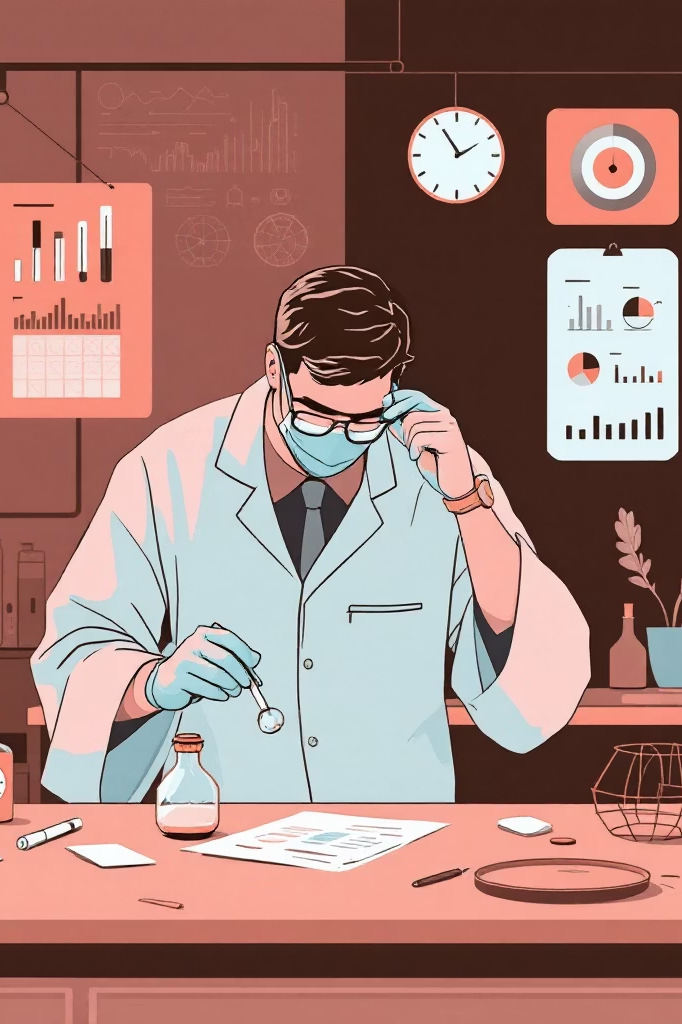
\includegraphics[width=\textwidth]{Figures/forense.png}
      \end{figure}
    \end{column}
  \end{columns}
\end{frame}

\section{Parte A -- Ley de Newton}
\begin{frame}
  \frametitle{Planteamiento (Parte A)}
  \begin{columns}
    \begin{column}{0.6\textwidth}
      \begin{itemize}
        \item Temperatura ambiente: $T_a=70^{\circ}\mathrm{F}$ (constante).
        \item Condici\'on inicial: $T(0)=98.6^{\circ}\mathrm{F}$ (momento de la muerte aproximado).
        \item Mediciones: $T(0)=80^{\circ}\mathrm{F}$ a las 12:00 y $T(1)=75^{\circ}\mathrm{F}$ a la 13:00.
      \end{itemize}
    \end{column}
    \begin{column}{0.4\textwidth}
      \begin{figure}
        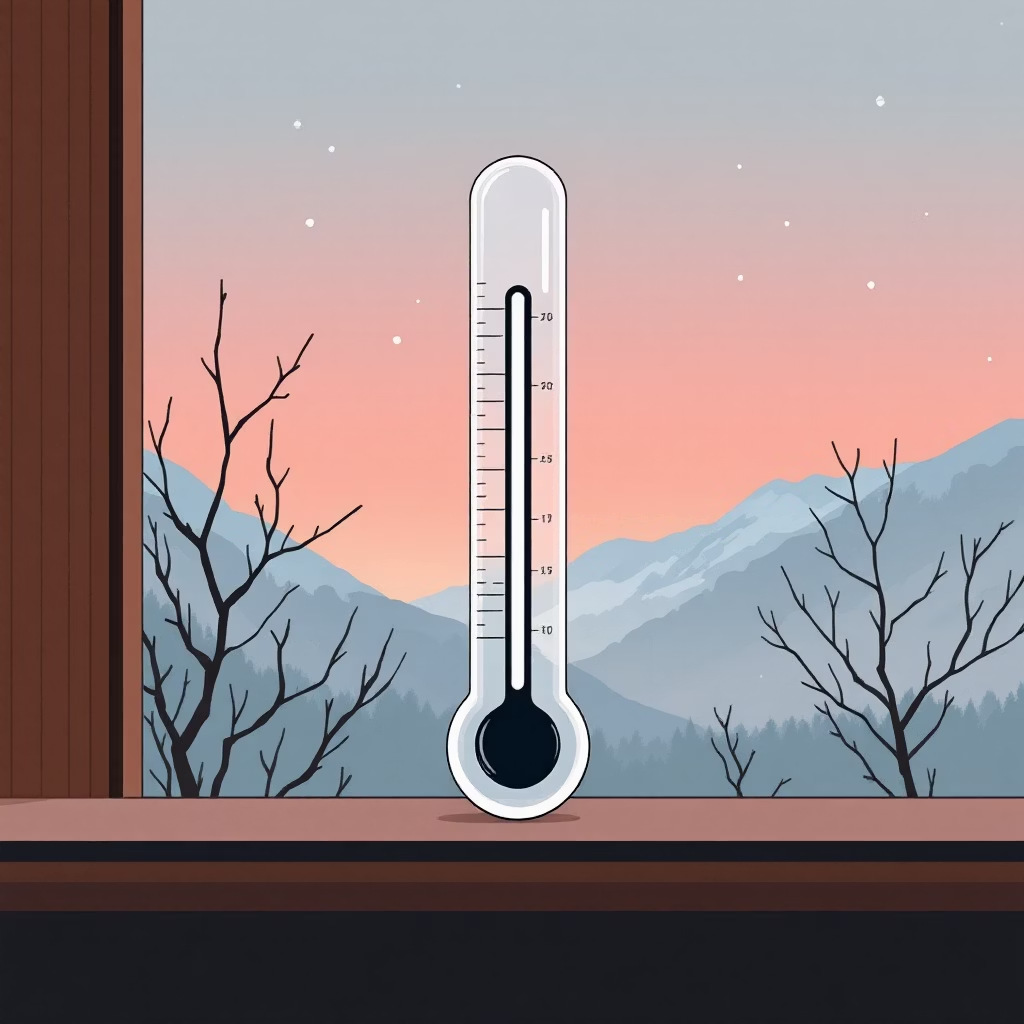
\includegraphics[width=0.8\textwidth]{Figures/termometer.png}
      \end{figure}
    \end{column}
  \end{columns}
\end{frame}

\begin{frame}
  \frametitle{Ecuaci\'on anal\'itica}
  Ley de Newton: $\dfrac{dT}{dt}=-k(T-T_a),\; k>0$.\\[6pt]
  Soluci\'on general: $T(t)=C e^{-kt}+T_a$.\\[6pt]
  Usando las mediciones se obtiene $C=10$ y
  \[\;T(t)=10e^{-kt}+70\;\].
  A partir de $T(1)=75$ se obtiene $e^{-k}=\tfrac{1}{2}$, luego
  \[\;k=\ln 2.\;\]
\end{frame}

\begin{frame}
  \frametitle{Estimaci\'on del tiempo de la muerte}
  \begin{columns}
    \begin{column}{0.65\textwidth}
      Para hallar $t$ cuando $T(t)=98.6$:\\[4pt]
      $\;98.6=10e^{-\ln(2)\,t}+70\Rightarrow e^{-\ln(2)\,t}=2.86\Rightarrow t= -\dfrac{\ln(2.86)}{\ln 2}\approx -1.515\,$ horas.\\[6pt]
      Interpretaci\'on: la muerte ocurri\'o aproximadamente $1.515$ h antes de las 12:00 (alrededor de las 10:29 AM).
    \end{column}
    \begin{column}{0.35\textwidth}
      \begin{figure}
        
\includegraphics[width=\textwidth]{Figures/clock.png}
      \end{figure}
    \end{column}
  \end{columns}
\end{frame}

\begin{frame}
  \frametitle{Comparaci\'on num\'erica (t=1 h)}
  \begin{tabular}{l c c}
    \hline
  M\'etodo & N & $T(1)$ ($^{\circ}\mathrm{F}$) \\
    \hline
    Anal\'itica & N/A & 75.000000 \\
    Euler & 1 & 74.741875 \\
    Euler Mejorado & 2 & 75.012333 \\
    \hline
  \end{tabular}
  \vspace{6pt}
  Observaci\'on: RK4 ofrece mayor precisi\'on; se calcul\'o el error absoluto y costo relativo en el reporte.
\end{frame}

\begin{frame}
  \frametitle{Isoclinas y campo de direcciones}
  \begin{figure}
    \centering
    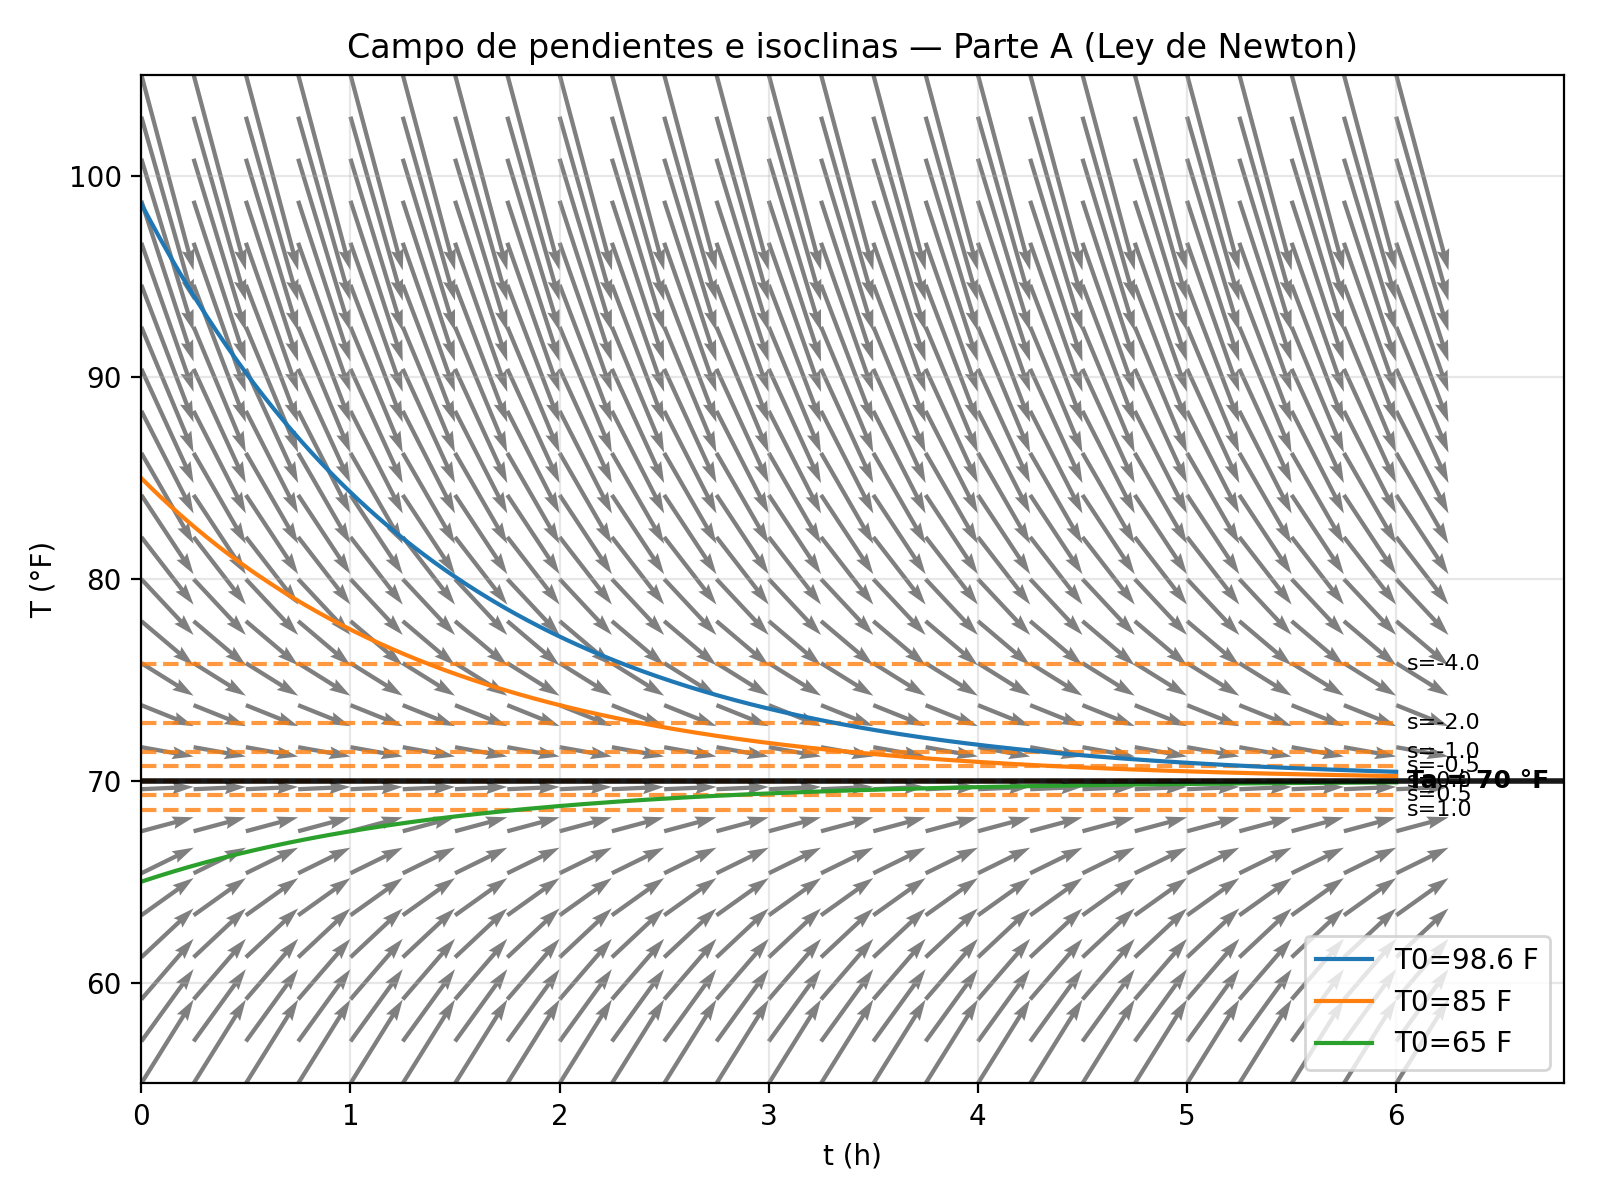
\includegraphics[width=0.7\textwidth]{Figures/isoclinas_partA.png}
    \caption{Visualizaci\'on de isoclinas para la Ley de Newton}
  \end{figure}
\end{frame}

\section{Parte B -- Bifurcaci\'on}
\begin{frame}
  \frametitle{Modelo (Parte B)}
  Estudiamos la EDO adimensional
  \[\;u' = \mu u + u^{3}, \quad \mu\in\mathbb{R}.\;\]
  Equilibrios: $u(\mu+u^{2})=0\Rightarrow u=0$ y $u=\pm\sqrt{-\mu}$ (estas aparecen solo si $\mu<0$).
\end{frame}

\begin{frame}
  \frametitle{An\'alisis de estabilidad y diagrama}
  Linealizando: $f'(u)=\mu+3u^{2}$.\\[4pt]
  - En $u=0$: $f'(0)=\mu$ \; (estable para $\mu<0$, inestable para $\mu>0$).\\
  - En $u=\pm\sqrt{-\mu}$ (si $\mu<0$): $f' = -2\mu>0$ (ramas no triviales inestables).\\[6pt]
  Interpretaci\'on: bifurcaci\'on tipo horquilla subcr\'itica en $\mu=0$ (las ramas no triviales colapsan en la trivial y son inestables).
\end{frame}

\begin{frame}
  \frametitle{Diagrama de bifurcaci\'on}
  \begin{figure}
    \centering
    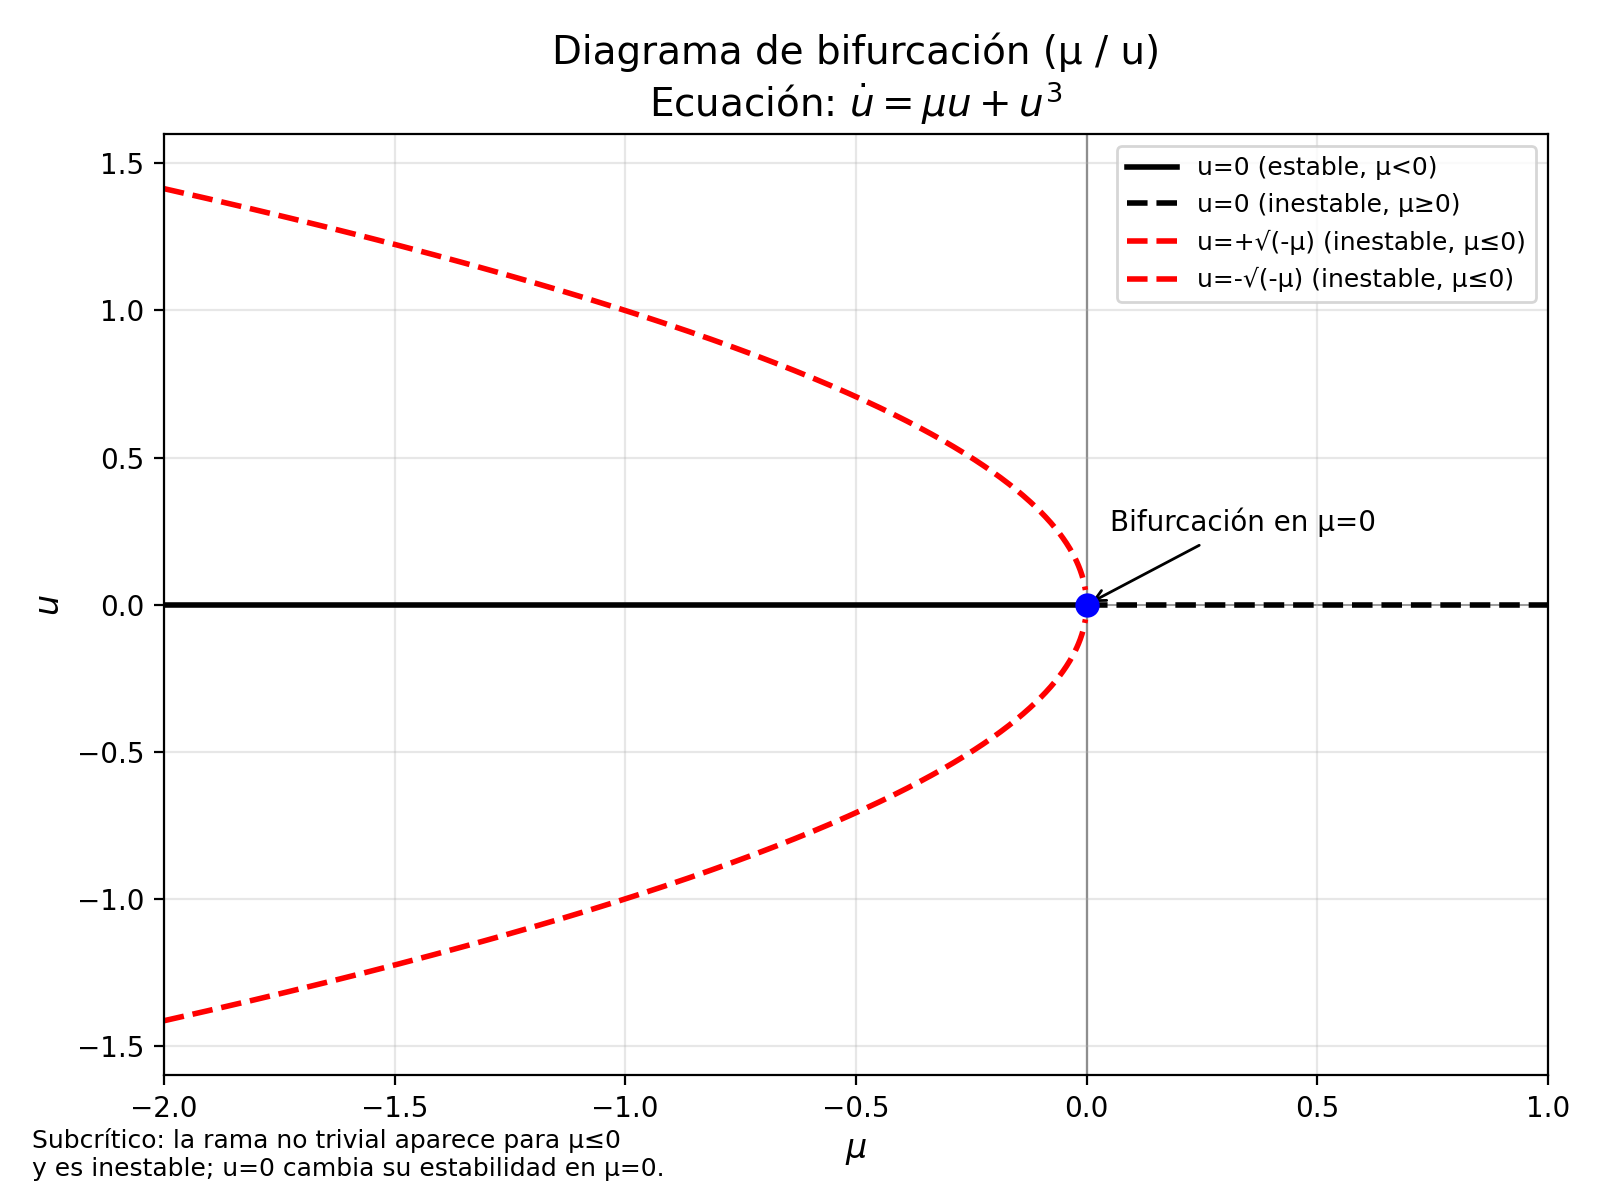
\includegraphics[width=0.75\textwidth]{Figures/bifurcation_mu_u.png}
    \caption{Diagrama de bifurcaci\'on para $u' = \mu u + u^{3}$}
  \end{figure}
\end{frame}

\section{Parte C -- Sistema 2-compartimentos}
\begin{frame}
  \frametitle{Planteamiento (Parte C)}
  Variables relativas: $x=X-A,\;y=Y-A$ con $A=70$. Sistema:
  \[\begin{cases}
     \dot x = -4(x-y),\\
     \dot y = -y.
  \end{cases}\]
  Se pide: puntos cr\'iticos, clasificaci\'on y significado f\'isico de las trayectorias.
\end{frame}

\begin{frame}
  \frametitle{Puntos cr\'iticos y matriz jacobiana}
  El \'unico punto cr\'itico es $(0,0)$. La forma matricial:
  \[\begin{pmatrix}\dot x\\\dot y\end{pmatrix} = \begin{pmatrix}-4 & 4\\0 & -1\end{pmatrix}\begin{pmatrix}x\\y\end{pmatrix}.
  \]
  Los autovalores se obtienen del polinomio caracter\'istico; en el reporte se realiza el c\'alculo espectral y la clasificaci\'on.
\end{frame}

\begin{frame}
  \frametitle{Plano de fase}
  \begin{figure}
    \centering
    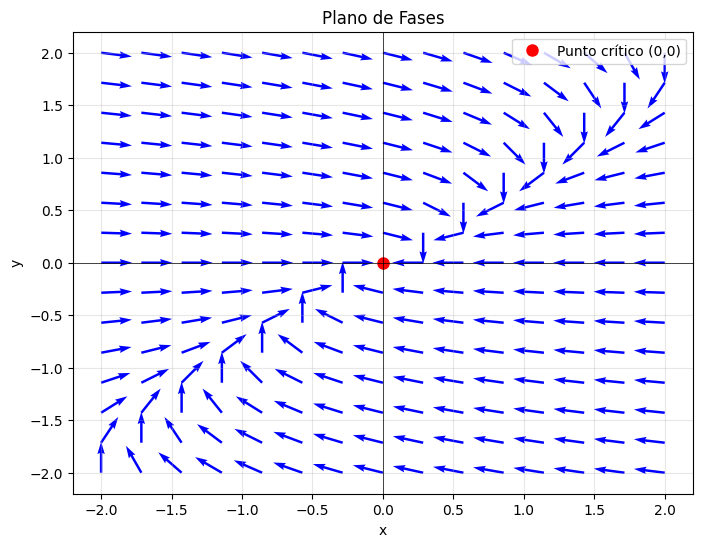
\includegraphics[width=0.7\textwidth]{Figures/plano_de_fase.png}
    \caption{Plano de fase del sistema de dos compartimentos}
  \end{figure}
\end{frame}

\begin{frame}
  \frametitle{Interpretaci\'on f\'isica}
  \begin{itemize}
    \item El sistema modela intercambio t\'ermico entre el n\'ucleo y la capa externa con disipaci\'on al ambiente.
    \item Las trayectorias en el plano de fase muestran relajaci\'on hacia el equilibrio $(0,0)$; la geometr\'ia de las trayectorias depende de los autovalores y vectores propios.
  \end{itemize}
\end{frame}

\begin{frame}
  \frametitle{Diagrama de fase detallado}
  \begin{figure}
    \centering
    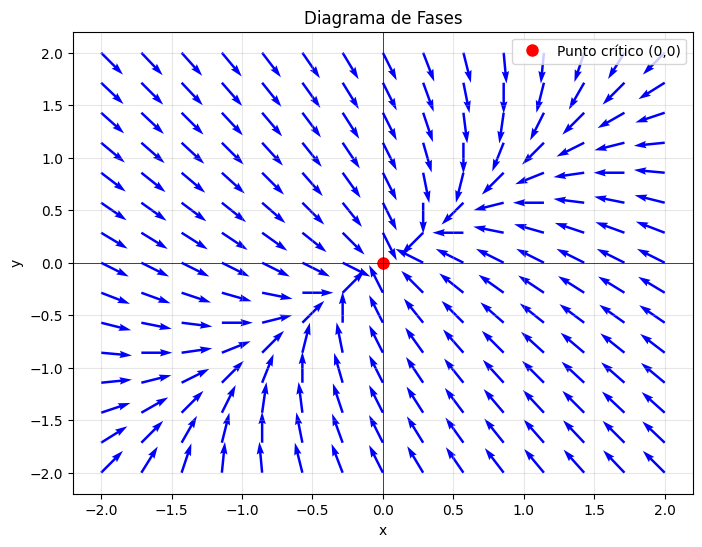
\includegraphics[width=0.7\textwidth]{Figures/phase_diagram.png}
    \caption{Diagrama de fase con trayectorias}
  \end{figure}
\end{frame}

\begin{frame}
  \frametitle{Conclusiones}
  \begin{itemize}
    \item La ley de Newton permite estimar el tiempo de la muerte con supuestos sencillos; en el ejemplo se obtiene ~1.515 h antes de las 12:00.
    \item El estudio cualitativo (isoclinas, campos de pendiente, bifurcaciones) aporta comprensión sobre cambios de r\'egimen.
    \item Comparaciones num\'ericas muestran que RK4 es preferible por precisi\'on/costo en estos ejemplos.
    \item Limitaciones: modelos simplificados, condiciones iniciales y homogeneidad; las aplicaciones forenses requieren validar supuestos y considerar incertidumbre.
  \end{itemize}
\end{frame}

\end{document}
